\documentclass[12pt,a4paper]{article}

% --- Packages ---
\usepackage[margin=1in]{geometry}
\usepackage{graphicx}
\usepackage{hyperref}
\usepackage{enumitem}
\usepackage{titlesec}
\usepackage{array}
\usepackage{xcolor}
\usepackage{booktabs}
\usepackage{longtable}
\usepackage{tabularx}
\usepackage{amsmath,amssymb}
\usepackage{siunitx}
\usepackage{multirow}
\usepackage{caption}
\usepackage{subcaption}
\usepackage{float}
\usepackage{listings}
\usepackage[ruled,vlined]{algorithm2e}
\usepackage{tikz}
\usepackage{fancyhdr} % header/footer control for small logo
\usetikzlibrary{arrows.meta,positioning,fit,calc,shapes.misc,shapes.geometric}

% --- Branding ---
\definecolor{brandblue}{RGB}{14,75,140}
\definecolor{brandgreen}{RGB}{25,135,84}
\definecolor{brandgray}{RGB}{90,90,100}

\hypersetup{
  colorlinks=true,
  linkcolor=brandblue,
  citecolor=brandblue,
  urlcolor=brandblue,
  pdftitle={PropVisions White Paper},
  pdfauthor={PropVisions},
  pdfsubject={The Complete AI-Powered Property Investment Platform}
}

\newcommand{\logoPath}{/Users/jamesquessy/Desktop/property-scout-ui/PropVisions_Logo.png}

% --- Section style ---
\titleformat{\section}{\color{brandblue}\normalfont\Large\bfseries}{}{0em}{}
\titleformat{\subsection}{\color{brandgreen}\normalfont\large\bfseries}{}{0em}{}
\titleformat{\subsubsection}{\color{brandgray}\normalfont\normalsize\bfseries}{}{0em}{}

% --- Listings (code blocks) ---
\lstset{
  basicstyle=\ttfamily\small,
  breaklines=true,
  frame=single,
  rulecolor=\color{brandgray},
  keywordstyle=\color{brandblue}\bfseries,
  commentstyle=\itshape\color{brandgreen},
  stringstyle=\color{brandblue},
  showstringspaces=false
}

\begin{document}

% ------------------------- COVER PAGE -------------------------
\begin{titlepage}
  \centering
  \vspace*{1.5cm}

  % Larger cover logo
  \includegraphics[width=0.65\textwidth]{\logoPath}

  \vspace{2.5cm}
  {\fontsize{28}{30}\selectfont\bfseries PropVisions\par}
  \vspace{0.6em}
  {\Large The Complete AI-Powered Property Investment Platform\par}

  \vspace{2.5cm}
  {\large White Paper\par}
  \vspace{0.4em}
  {\normalsize Version 1.0 \quad | \quad Confidential Draft for Early Partners and Reviewers\par}

  \vfill
  \color{brandgray}
  \rule{\textwidth}{0.6pt}\par
  \vspace{0.6em}
  {\small Last updated: \today \quad • \quad \textcolor{brandblue}{\href{https://www.propvisions.com}{www.propvisions.com}} \quad • \quad hello@propvisions.com\par}
\end{titlepage}

% ------------------------- HEADER WITH SMALL LOGO -------------------------
\pagestyle{fancy}
\fancyhf{}
\setlength{\headheight}{20pt}
\renewcommand{\headrulewidth}{0pt}
\fancyhead[L]{\textbf{\color{brandblue}PropVisions}\\\small White Paper}
\fancyhead[R]{\raisebox{-0.2\height}{\includegraphics[height=14mm]{\logoPath}}} % increased to 14mm
\fancyfoot[C]{\thepage}

% ------------------------- FRONT MATTER -------------------------
\pagenumbering{roman}
\setcounter{page}{1}

\tableofcontents
\newpage

% Switch to arabic numbering for the main body
\pagenumbering{arabic}
\setcounter{page}{1}

% =========================================================
\section{Executive Summary}
\textbf{PropVisions} is an AI-first property investment platform that automates the end-to-end lifecycle of sourcing, underwriting, reporting, and monitoring UK residential deals. The system combines: robust ingestion from URLs/APIs; computer-vision-driven refurbishment estimation from listing photos; rent band forecasting using historical data and listing signals; full-stack financials; EPC enrichment; comparables sanity checks; high-quality PDF/Excel outputs; and ongoing alerts post-purchase (rates, remortgage timing, deal-status changes).

\paragraph{What this document covers.} Current MVP and near-term roadmap, reference architecture, canonical schemas, algorithms, operational controls, security \& GDPR posture, evaluation methodology, commercialization path, and pilot structure.

\paragraph{Positioning.} Unlike calculators or point tools, PropVisions provides: (i) automated upstream data capture, (ii) transparent, AI-assisted analysis with human-in-the-loop overrides, and (iii) post-purchase monitoring—forming a continuous improvement loop.

\paragraph{Outcome.} Reduce analysis time from hours to minutes; standardise underwriting; deliver client-ready packs; and scale to hundreds of deals per analyst per week with auditable assumptions.

% =========================================================
\section{Beta Status and Transparency}
\textbf{Active beta.} Fast progress; imperfect outputs. UI is practical-first. Accuracy is variable by area and listing quality. We publish baseline accuracy metrics and expose confidence bands and editable assumptions.

\begin{itemize}[leftmargin=1.5em]
  \item \textbf{Target accuracy (near-term):} rent band hit-rate $\geq 80\%$; refurb total MAPE $\leq 20$--$25\%$ with 10+ images; EPC match $\geq 95\%$ on clean addresses.
  \item \textbf{Levers you can edit:} management\%, voids, maintenance, fees, growth assumptions, refurb line items, rent bands.
  \item \textbf{Human judgement remains central:} we provide structure, speed, and signal—not guarantees.
\end{itemize}

% =========================================================
\section{Product Overview}
\subsection{Elevator Pitch}
Paste a property link (or run a saved search) and PropVisions outputs a complete investment snapshot—refurb costs by room, rent band with confidence, yield/ROI/cashflow, EPC, comps, and report files—then watches for updates (price drops, back-on-market, remortgage windows) and alerts you.

\subsection{What Works Today (MVP)}
\begin{enumerate}[leftmargin=1.5em]
  \item \textbf{URL ingestion} $\rightarrow$ scrape \& parse: price, address/postcode, layout, features, images, agent details.
  \item \textbf{Refurb from photos} (vision-guided): per-room items; regional cost indices; editable totals \& contingencies.
  \item \textbf{Rent estimation:} historical rent data + listing features $\rightarrow$ monthly/annual band with rationale \& confidence.
  \item \textbf{Financials:} stamp duty, legal/survey/insurance, management\%, voids, maintenance \textrightarrow{} yield, ROI, cashflow.
  \item \textbf{EPC enrichment:} rating \& recommended measures; record stored for reporting.
  \item \textbf{Comps sanity checks:} recent locals; £/sqft bands; outlier flags.
  \item \textbf{Outputs \& alerts:} PDF/Excel; Slack/email notification with links.
\end{enumerate}

\subsection{Planned Features (Highlights)}
\begin{itemize}[leftmargin=1.5em]
  \item \textbf{Unified search \& APIs:} Rightmove, Zoopla, OnTheMarket, auction platforms; de-dup, canonicalisation, watchlists.
  \item \textbf{Deal-status watcher:} new/returning, price drops, time-on-market; filters by postcode/price/bed/yield/refurb budget.
  \item \textbf{Mortgage module:} product types (IO/repayment), fees/ERCs, ICR/DSCR, forward curve scenarios, remortgage assistant.
  \item \textbf{Portfolio \& sharing:} multi-deal comparisons, read-only client views, white-label branding.
  \item \textbf{Off-market assistants:} GDPR-compliant outreach, probate/distress signals, light CRM for cadence tracking.
\end{itemize}

% =========================================================
\section{Design Principles \& Defaults}
\begin{itemize}[leftmargin=1.5em]
  \item \textbf{Transparency over black-box:} show bands, confidence, and levers; capture overrides and provenance.
  \item \textbf{Speed with correctness:} deterministic parsers \& validations first; LLMs only where they add value.
  \item \textbf{Local realism:} regional cost indices for refurb; postcode priors for rent.
  \item \textbf{Secure by default:} least-privilege, audited access, encrypted storage, no secrets in code.
  \item \textbf{Human-in-the-loop:} every estimate is editable; edits feed calibration.
\end{itemize}

% =========================================================
\section{User Personas \& Jobs-To-Be-Done}
\subsection{Professional Investor}
\textit{JTBD:} underwrite consistently; generate investor packs; track portfolio KPIs; spot remortgage opportunities.

\subsection{Sourcing Agent}
\textit{JTBD:} scan many deals; qualify quickly; package for buyers with credible numbers; automate alerts.

\subsection{Estate Agency / Partner}
\textit{JTBD:} add value to buyers with analytics; white-label reports; evidence-based pricing; improve conversion.

% =========================================================
\section{System Architecture}
\subsection{High-Level Diagram}
\begin{figure}[H]
\centering
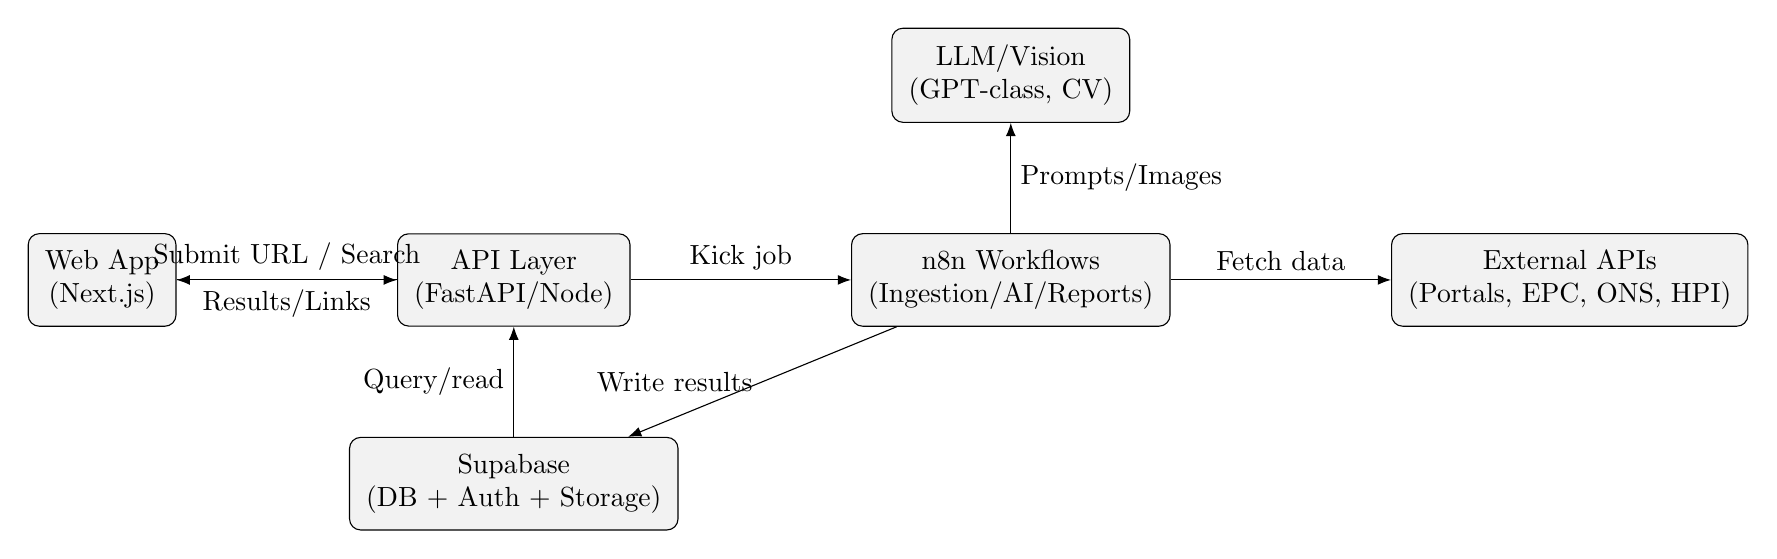
\begin{tikzpicture}[node distance=1.4cm,>=Latex]
\tikzstyle{box}=[draw, rounded corners, align=center, inner sep=6pt]
\node[box, fill=gray!10] (user) {Web App \\ (Next.js)};
\node[box, right=2.8cm of user, fill=gray!10] (api) {API Layer \\ (FastAPI/Node)};
\node[box, right=2.8cm of api, fill=gray!10] (n8n) {n8n Workflows \\ (Ingestion/AI/Reports)};
\node[box, below=1.4cm of api, fill=gray!10] (db) {Supabase \\ (DB + Auth + Storage)};
\node[box, above=1.4cm of n8n, fill=gray!10] (models) {LLM/Vision \\ (GPT-class, CV)};
\node[box, right=2.8cm of n8n, fill=gray!10] (ext) {External APIs \\ (Portals, EPC, ONS, HPI)};

\draw[->] (user) -- (api) node[midway, above]{Submit URL / Search};
\draw[->] (api) -- (n8n) node[midway, above]{Kick job};
\draw[->] (n8n) -- (models) node[midway, right]{Prompts/Images};
\draw[->] (n8n) -- (ext) node[midway, above]{Fetch data};
\draw[->] (n8n) -- (db) node[midway, left]{Write results};
\draw[->] (db) -- (api) node[midway, left]{Query/read};
\draw[->] (api) -- (user) node[midway, below]{Results/Links};
\end{tikzpicture}
\caption{PropVisions high-level architecture.}
\end{figure}

\subsection{Workflow Orchestration (n8n)}
\begin{enumerate}[leftmargin=1.5em]
  \item \textbf{Scrape Node:} fetch HTML/media with retries, backoff, \& robots/T\&Cs respect.
  \item \textbf{Clean \& Parse:} deterministic selectors + LLM cleanup; strong schema validation.
  \item \textbf{Image Loop:} refurb agent per image; classify room, extract conditions; aggregate by room type.
  \item \textbf{Rent Agent:} regression prior + LLM adjustment (listing text, amenities, finish).
  \item \textbf{Fees \& ROI:} stamp duty, legal, insurance, mgmt, maintenance, voids; yield, ROI, cashflow.
  \item \textbf{HPI/Uplift:} baseline growth; optional AI uplift vs comps; sensitivity ranges.
  \item \textbf{EPC Match:} heuristic + LLM fallback; store matched record + recommended measures.
  \item \textbf{Reporting:} render PDF/Excel; upload artifacts; generate share links.
  \item \textbf{Notify:} Slack/email with KPIs and download URLs.
\end{enumerate}

\subsection{Data Stores}
\textbf{Supabase Postgres:} canonical tables for properties, analyses, refurb/rent/EPC/comps, runs, and reports. \\
\textbf{Supabase Storage:} artifact storage (PDF/Excel). \\
\textbf{Auth:} users, teams, roles; future SSO.

% =========================================================
\section{Canonical Schemas (Selected)}
\subsection{Core Entities}
\begin{longtable}{@{}p{3.2cm}p{12.4cm}@{}}
\toprule
\textbf{Table} & \textbf{Purpose \& Key Fields} \\
\midrule
\texttt{properties} & Canonical property identity. \textit{Fields:} id, url, address\_full, postcode, source, first\_seen, last\_seen, status, agent jsonb. \\
\texttt{analyses} & One analysis per run/version. \textit{Fields:} id, property\_id, run\_timestamp, price, layout jsonb, assumptions jsonb, results jsonb, confidence jsonb. \\
\texttt{refurb\_estimates} & Room-/item-level refurb costs. \textit{Fields:} id, analysis\_id, room\_type, items jsonb, subtotal, contingency, confidence. \\
\texttt{rent\_estimates} & Rent predictions and sources. \textit{Fields:} id, analysis\_id, monthly\_rent, band\_low, band\_high, method, comps jsonb, confidence, rationale text. \\
\texttt{sales\_comps} & Nearby sales comparables. \textit{Fields:} address, distance\_m, price, date, sqft, ppsf, weight. \\
\texttt{rental\_comps} & Nearby rental comparables. Similar to sales comps, with monthly rent. \\
\texttt{epc\_records} & EPC details. \textit{Fields:} rating, uprn, lmk\_key, measures jsonb, full\_record jsonb. \\
\texttt{reports} & Generated artifacts. \textit{Fields:} type (pdf/xlsx), storage\_path, size\_bytes, checksum. \\
\texttt{runs} & Orchestration metadata. \textit{Fields:} workflow\_id, duration\_ms, status, error\_log, tokens\_used. \\
\bottomrule
\end{longtable}

% =========================================================
\section{Algorithms \& Methods}
\subsection{HTML $\rightarrow$ JSON Extraction}
Deterministic tag/attribute rules to collect candidates (price, address, beds/baths, agent, features), then an LLM cleans/standardises. Ambiguity yields warnings; never fabricate. \textbf{Validation:} regex \& unit checks, currency normalisation, postcode parsing, and required-field gating.

\subsection{Vision-Guided Refurb Estimation}
\textbf{Input:} photos (kitchen, bathroom, bedroom, lounge, hallway, exterior). \\
\textbf{Pipeline:}
\begin{enumerate}[leftmargin=1.5em]
  \item \textbf{Room classification} (CV cues + prompt heuristics).
  \item \textbf{Condition extraction} (cabinet age, tiles, damp marks, flooring wear).
  \item \textbf{Bill-of-quantities map} (replace cabinets, re-tile, rewire room, paint, flooring).
  \item \textbf{Regional cost index} by postcode; labour/material splits.
  \item \textbf{Confidence scoring} and \textbf{contingency} policy (e.g., 10--15\%).
\end{enumerate}

\subsection{Rent Estimation (Hybrid)}
Regression prior on postcode + features (\emph{beds, type, EPC, finish proxies}) blended with LLM adjustment from listing signals:
\[
\hat{R} = \alpha R_{\text{prior}} + (1-\alpha)R_{\text{LLM}},\quad \alpha \in [0.5, 0.8] \text{ by region}
\]
Band and confidence reflect historical dispersion and text cues.

\subsection{EPC Matching (Heuristic + Fallback)}
Normalise strings; extract house number \& street tokens; filter exact postcode; score candidates with house\# match, Jaccard of street tokens, and edit distance; threshold or null. Fallback LLM comparison if borderline.

\subsection{Financials \& Mortgage}
Given price $P$, refurb $C_r$, other fees $F$, annual rent $R_a$, expense ratio $e$, mgmt $\mu$:
\[
\text{NOI} = R_a(1 - e - \mu),\quad
\text{Yield} = \frac{\text{NOI}}{P + C_r + F}
\]
Mortgage cashflow with amortisation or IO; ICR/DSCR computed against stressed rates; sensitivity tables across rates and voids.

\subsection{Uplift \& Forecasting}
Baseline HPI growth and comparable uplift $\Delta$:
\[
P' = (P + C_r)(1 + g_{\text{HPI}}) + \Delta
\]
Scenarios sweep $g_{\text{HPI}}$, rent, and refurb to produce tornado/range outputs in Excel/PDF.

% =========================================================
\section{Prompts \& Guardrails}
\subsection{Strict JSON Output Guard (Global)}
\begin{lstlisting}
System: Output only VALID JSON. No markdown, no comments. If unsure, use null.
User: If any schema key is missing, include it with null. Prefer empty arrays to missing arrays.
\end{lstlisting}

\subsection{HTML-to-JSON}
\begin{lstlisting}
System: You are a strict data extractor. If a field is unknown, return null.
User: Given raw HTML and images, return ONLY:
{price_gbp, address, postcode, bedrooms, bathrooms, tenure, agent, features[]}
Do not invent values. If ambiguous, set null and add "warnings":[...].
\end{lstlisting}

\subsection{Refurb (Vision)}
\begin{lstlisting}
System: Estimate refurbishment line-items from photos using UK trade assumptions.
User: For each image: classify room; list items {category, qty, unit, unit_rate_gbp, subtotal_gbp}.
Adjust for postcode cost index if provided. Return JSON only with a "confidence" 0..1.
\end{lstlisting}

\subsection{Rent}
\begin{lstlisting}
System: Estimate monthly rent (GBP) given features + listing text cues.
User: Return:
{ monthly_rent_gbp, low, high, rationale, confidence }
Do not exceed local comparables by >15% without explicit justification.
\end{lstlisting}

\subsection{EPC Fallback}
\begin{lstlisting}
System: Match a single EPC record to title+postcode and return exactly one JSON object.
User: Inputs: propertyTitle, postcode, epcRecords[]. If unsure, return nulls (no guess).
\end{lstlisting}

% =========================================================
\section{Evaluation \& Accuracy}
\subsection{Metrics}
\begin{itemize}[leftmargin=1.5em]
  \item \textbf{Rent MAE/MAPE} vs let-agreed.
  \item \textbf{Refurb error} vs invoices or QS estimates (room bundle and total).
  \item \textbf{EPC precision/recall} on labelled set.
  \item \textbf{Deal error} in Year-1 net yield and cashflow.
\end{itemize}

\subsection{Targets (Beta)}
\begin{itemize}[leftmargin=1.5em]
  \item Rent MAPE: 10--15\% (1--2 bed flats); 15--20\% mixed stock.
  \item Refurb: 20--30\% total; 15--25\% with $>$10 images.
  \item EPC: $>$95\% precision on clean data; $>$90\% otherwise.
  \item Net yield error: $\pm(1$--$1.5)$pp for standard BTL scenarios.
\end{itemize}

\subsection{Protocol}
Hold-out by region \& type; backtest against outcomes; publish aggregate, regional, and dispersion stats; monitor monthly drift.

% =========================================================
\section{Security, Compliance, and Data Governance}
\subsection{GDPR}
Lawful bases (Legitimate Interests/Contract); data minimisation (only needed fields); opt-in flows for outreach; DPA on request; DPIA maintained.

\subsection{Credentials \& Secrets}
Env vars/secret managers; never in code or reports; rotated; least-privilege access; redaction in logs.

\subsection{PII \& Retention}
Default retention 12 months (configurable); right-to-erasure; access logging; subject access workflows.

% =========================================================
\section{Performance, Reliability \& Cost}
\subsection{Latency Budgets}
\begin{itemize}[leftmargin=1.5em]
  \item End-to-end target: 30--90s per property (image count dependent).
  \item HTML parse $<$ 3s; image loop $<$ 40s (10--15 images); EPC/API $<$ 5s; PDF/Excel $<$ 7s.
\end{itemize}

\subsection{COGS (Illustrative)}
LLM tokens across parse/images/rent/EPC: \pounds0.05--\pounds0.20; storage pennies per artifact; typical run \pounds0.10--\pounds0.40 (model/volume dependent). Caching, heuristics, and smaller models reduce cost at scale.

\subsection{Reliability}
Retries with backoff; circuit breakers on third-party APIs; idempotent writes; run journaling; dead-letter queues; error budgets and SLOs.

% =========================================================
\section{Commercial Strategy}
\subsection{Pricing (Indicative)}
\begin{itemize}[leftmargin=1.5em]
  \item \textbf{Starter:} \pounds29/mo, 50 runs; \pounds1/run overage.
  \item \textbf{Pro:} \pounds99/mo, 300 runs; team seats; alerts; branded outputs.
  \item \textbf{Team/Agency:} \pounds299+/mo, 1000 runs; SSO; white-label; priority support.
  \item \textbf{Custom Regions:} one-off setup + premium monthly; accuracy guarantees in coverage zones.
\end{itemize}

\subsection{GTM}
Beta cohort (10--20 users) with discounted lifetime tiers; partnerships with sourcing groups \& agents; thought leadership (accuracy dashboards, regional insights); demo tours and case studies.

\subsection{Unit Economics}
Gross margin $>$80\% at scale; levers: prompt efficiency, model choice, deduped runs, batch scoring, regional fine-tunes.

% =========================================================
\section{Operational Playbooks}
\subsection{Incident Response}
Severity P1 (platform down), P2 (module degraded), P3 (single-integration issue). On-call rotation; status page; user comms templates; post-mortems within 72h.

\subsection{Monitoring \& Observability}
Run-level tracing (IDs across scrape/AI/report); latency histograms; token usage; error rates by node; alerting thresholds per integration.

\subsection{Data Quality Gates}
Schema validators; required-field gates; unit/currency checks; postcode validators; numerical bounds; \textit{warnings[]} propagated into UI/report.

% =========================================================
\section{Mortgage Module (Now \& Next)}
\subsection{MVP}
Standard assumptions (rates, LTV, product fee) included in cashflow and ROI; IO vs repayment switch; ICR check.

\subsection{Next}
Product matrices; ERC modelling; fee amortisation; forward curve scenarios; remortgage window alerts based on LTV and rate environment; DSCR/ICR charting in dashboard.

% =========================================================
\section{Deal Discovery \& Off-Market}
\subsection{Watchers}
New listings, price changes, back-on-market; filters across location/price/bed/yield/refurb-budget; digest emails/Slack.

\subsection{Off-Market Assistant}
GDPR-compliant outreach templates; agent cadence trackers; probate/distress signals where available; lightweight CRM to log replies and next actions.

% =========================================================
\section{Roadmap (Detailed)}
\subsection{Weeks 1--6 (MVP Polishing)}
\begin{longtable}{@{}p{2cm}p{13.6cm}@{}}
\toprule
\textbf{Week} & \textbf{Objectives} \\
\midrule
1 & Harden scraper; HTML$\to$JSON prompt v2; finalise canonical schemas; seed postcode priors. \\
2 & Vision refurb v2 (better room detection); regional cost indices; contingency policy. \\
3 & Rent hybrid v2; band confidence; export PDF/Excel v1. \\
4 & EPC matcher v2; comps sanity checks; warnings pipeline; Slack/email alert polish. \\
5 & Dashboard polish; scenario inputs; share links; onboarding walkthrough. \\
6 & Stress tests; logging/observability; beta onboarding and support playbooks. \\
\bottomrule
\end{longtable}

\subsection{Launch (v1)}
Unified search; API connectors (portals/auctions); de-dup \& canonicalisation; batch imports; saved searches; error dashboards; accuracy baselines published.

\subsection{Q2}
Watchers and off-market module; smarter comps; regional calibration; push rent-band hit-rate; reduce refurb variance; client-shareable read-only dashboards.

\subsection{Q3}
Mortgage types \& forward curves; live scenario dashboard; remortgage assistant; DSCR/ICR visuals; accuracy bands shrink with feedback.

\subsection{Q4}
White-label/embeddable widgets; team workflows; advanced portfolio analytics; acquisition-readiness hardening.

% =========================================================
\section{Risk Register \& Mitigations}
\begin{longtable}{@{}p{3cm}p{7.5cm}p{4.5cm}@{}}
\toprule
\textbf{Risk} & \textbf{Description} & \textbf{Mitigation} \\
\midrule
Data drift & Rents/refurb costs shift regionally. & Monthly backtests; retrain priors; user feedback weighting. \\
API fragility & Portal/third-party API changes. & Abstraction layer; fallback scrapers; monitoring \& alerts. \\
LLM variability & Output changes across versions. & Strict schemas; retries; guardrails; cache; unit tests on prompts. \\
Compliance & Outreach \& data usage. & GDPR DPIA; opt-in; audit logs; DPA; rate-limiting. \\
COGS creep & Token costs increase. & Smaller models; heuristics; caching; batch operations. \\
\bottomrule
\end{longtable}

% =========================================================
\section{Case Study (Illustrative)}
\subsection{Deal Summary}
Guide price \pounds525k; 2-bed flat; W2 postcode. Refurb: kitchen refresh, bathroom mid-grade, redecoration. Rent estimate \pounds2{,}650/mo (low \pounds2{,}450, high \pounds2{,}850).

\subsection{Outputs}
Year-1 net yield 4.9\% (no leverage); leveraged ROI 6.8\%; uplift +\SI{6.5}{\percent}; EPC C; PDF with breakdowns; Slack alert to buyer and agent.

% =========================================================
\section{Support, SLAs, and Operations}
\subsection{Beta Support}
Email/Slack within 24h; incident comms; weekly build notes; in-product feedback capture; per-user accuracy scorecards.

\subsection{SLA Targets (Post-Beta)}
99.5\% uptime; P1 $<$ 4h mitigate; P2 $<$ 1 business day; monthly availability reports; RCA on P1/P2.

% =========================================================
\section{Conclusion}
PropVisions delivers a transparent, automation-first approach to deal analysis: fast ingestion, structured outputs, editable assumptions, and continuous monitoring. With disciplined execution, the platform aims to be the operating system for UK residential investors, sourcing agents, and partner estate agencies.

% =========================================================
\appendix
\section*{Appendix A: Supabase SQL DDL (Selected)}
\addcontentsline{toc}{section}{Appendix A: Supabase SQL DDL (Selected)}
\begin{lstlisting}[language=SQL]
-- Note: tighten types/constraints per environment.
create table public.properties (
  id uuid primary key default gen_random_uuid(),
  url text not null,
  address_full text,
  postcode text,
  source text,
  agent jsonb,
  first_seen timestamptz default now(),
  last_seen timestamptz default now(),
  status text default 'active'
);

create table public.analyses (
  id uuid primary key default gen_random_uuid(),
  property_id uuid references public.properties(id) on delete cascade,
  run_timestamp timestamptz default now(),
  price numeric,
  layout jsonb,
  assumptions jsonb not null default '{}',
  results jsonb not null default '{}',
  confidence jsonb not null default '{}'
);

create table public.refurb_estimates (
  id uuid primary key default gen_random_uuid(),
  analysis_id uuid references public.analyses(id) on delete cascade,
  room_type text,
  items jsonb not null,
  subtotal numeric,
  contingency numeric,
  confidence numeric
);

create table public.rent_estimates (
  id uuid primary key default gen_random_uuid(),
  analysis_id uuid references public.analyses(id) on delete cascade,
  monthly_rent numeric,
  band_low numeric,
  band_high numeric,
  method text,
  comps jsonb,
  confidence numeric,
  rationale text
);

create table public.epc_records (
  id uuid primary key default gen_random_uuid(),
  analysis_id uuid references public.analyses(id) on delete cascade,
  rating text,
  uprn text,
  lmk_key text,
  measures jsonb,
  full_record jsonb
);

create table public.reports (
  id uuid primary key default gen_random_uuid(),
  analysis_id uuid references public.analyses(id) on delete cascade,
  type text check (type in ('pdf','xlsx')),
  storage_path text not null,
  size_bytes bigint,
  checksum text,
  created_at timestamptz default now()
);
\end{lstlisting}

\section*{Appendix B: n8n Workflow (Pseudo-YAML)}
\addcontentsline{toc}{section}{Appendix B: n8n Workflow (Pseudo-YAML)}
\begin{lstlisting}
nodes:
  - Webhook: trigger { url, userId }
  - HTTP: fetch HTML (retries/backoff)
  - Code: sanitize & canonicalize URL
  - Agent: clean HTML -> JSON (price, address, features)
  - Loop: images[]
      - Agent: refurb estimate per image
  - Code: aggregate refurb lines -> totals + contingency
  - Agent: rent estimate (priors + listing signals)
  - Code: fees, mgmt, voids, maintenance, ROI
  - HTTP: HPI fetch -> uplift baseline
  - HTTP: EPC API -> candidate records
  - Agent: EPC match -> rating + record
  - PDF: compose report
  - Excel: compose spreadsheet
  - Supabase: upsert all tables
  - Slack: send summary + links
\end{lstlisting}

\section*{Appendix C: Report Structure (PDF/Excel)}
\addcontentsline{toc}{section}{Appendix C: Report Structure (PDF/Excel)}
\textbf{PDF:} Cover $\rightarrow$ KPI summary $\rightarrow$ Financials $\rightarrow$ Refurb (room items \& totals) $\rightarrow$ Rent \& comps $\rightarrow$ EPC $\rightarrow$ Forecasts $\rightarrow$ Assumptions \& Warnings $\rightarrow$ Disclaimer. \\
\textbf{Excel:} Tabs: Summary, Inputs, Refurb, Rent, Fees, EPC, Forecasts, Comps, Audit.

\section*{Appendix D: API Stubs (FastAPI)}
\addcontentsline{toc}{section}{Appendix D: API Stubs (FastAPI)}
\begin{lstlisting}[language=Python]
from fastapi import FastAPI, HTTPException
from pydantic import BaseModel
import uuid

app = FastAPI()

class RunRequest(BaseModel):
    url: str
    user_id: str

class RunResponse(BaseModel):
    job_id: str
    status: str

@app.post("/analyze", response_model=RunResponse)
def analyze(req: RunRequest):
    job_id = str(uuid.uuid4())
    # enqueue n8n webhook here
    return RunResponse(job_id=job_id, status="queued")
\end{lstlisting}

\section*{Appendix E: Prompt Library (Copy-Paste Ready)}
\addcontentsline{toc}{section}{Appendix E: Prompt Library (Copy-Paste Ready)}
\subsection*{Strict JSON Output Guard}
\begin{lstlisting}
System: Output only VALID JSON. No markdown, no comments. If unsure, use null.
If any schema key is missing, add it with null.
\end{lstlisting}

\subsection*{EPC Match (Final)}
\begin{lstlisting}
System: You are a deterministic matcher. Do not guess.
User: Inputs: { "propertyTitle": "...", "postcode": "...", "epcRecords": [...] }
Rules: normalise strings; exact postcode match required; penalise house-number mismatch;
if none cross a confidence threshold, return matched_epc: null, epc_rating: null.
Output schema:
{
  "property_title": "...",
  "postcode": "...",
  "matched_epc": { ... } | null,
  "epc_rating": "A"|"B"|...|null
}
\end{lstlisting}

\section*{Appendix F: Glossary}
\addcontentsline{toc}{section}{Appendix F: Glossary}
\begin{itemize}[leftmargin=1.5em]
  \item \textbf{EPC:} Energy Performance Certificate.
  \item \textbf{HPI:} House Price Index.
  \item \textbf{ICR/DSCR:} Interest Coverage / Debt Service Coverage Ratios.
  \item \textbf{MAPE:} Mean Absolute Percentage Error.
  \item \textbf{NOI:} Net Operating Income.
\end{itemize}

\end{document}
